% Created 2025-12-19 Fri 23:15
% Intended LaTeX compiler: pdflatex
\documentclass[11pt]{article}
\usepackage[utf8]{inputenc}
\usepackage[T1]{fontenc}
\usepackage{graphicx}
\usepackage{longtable}
\usepackage{wrapfig}
\usepackage{rotating}
\usepackage[normalem]{ulem}
\usepackage{amsmath}
\usepackage{amssymb}
\usepackage{capt-of}
\usepackage{hyperref}
\usepackage{subcaption}
\date{\today}
\title{}
\hypersetup{
 pdfauthor={},
 pdftitle={},
 pdfkeywords={},
 pdfsubject={},
 pdfcreator={Emacs 30.2 (Org mode 9.7.11)}, 
 pdflang={English}}
\begin{document}

\tableofcontents

\section{Abstract}
\label{sec:org00dd48d}

Quantum state denoising—reconstructing clean density matrices from noisy measurements—is essential for extracting useful information from near-term quantum devices. While prior work has explored convolutional and feedforward architectures for this task, the effectiveness of global attention mechanisms for quantum states with non-local entanglement correlations remains underexplored. We compare multilayer perceptron (MLP) and Transformer autoencoders for density matrix denoising, using comparable parameter counts (\textasciitilde{}120k) to reduce confounding from model capacity. On a synthetic dataset of 5-qubit states corrupted by five noise types at four severity levels, both models improve upon the baseline: the MLP achieves 1.4× higher Uhlmann fidelity while the Transformer achieves 2.3×—a 1.6× advantage over the MLP. We attribute this gap to the self-attention mechanism's ability to model correlations between arbitrary matrix elements. Our experiments also demonstrate that unconstrained outputs with post-hoc projection to valid density matrices enable effective optimization, whereas hard constraints (Cholesky parameterization) presented significant optimization difficulties in our configuration. These findings suggest that architectural choice—not merely model capacity—influences denoising performance for entangled quantum states.
\section{Introduction}
\label{sec:org82ba752}
Prior work has explored convolutional architectures for quantum state denoising, leveraging locally structured patterns induced by density-matrix representations to mitigate the effects of decoherence without assuming explicit knowledge of the underlying hardware noise channel (Karan Kendre, 2025). Earlier approaches employ feedforward neural networks to reconstruct states corrupted by unknown dynamics, demonstrating that supervised neural models can learn effective, data-driven mappings from noisy to cleaner quantum states (Morgillo, Angela Rosy and Mangini, Stefano and Piastra, Marco and Macchiavello, Chiara, 2024). However, these architectures process density matrices as flat vectors or local patches, potentially failing to capture the non-local correlations induced by quantum entanglement—a limitation that motivates exploring attention-based alternatives.

Beyond state-level denoising, machine learning has been widely applied to quantum error correction and control. Classical convolutional decoders (Breuckmann, Nikolas P. and Ni, Xiaotong, 2018) and multilayer perceptron models (Chamberland, Christopher and Ronagh, Pooya, 2018) have been trained on local stabilizer syndrome neighborhoods, but this approach limits scalability and often necessitates retraining when code distances change. Transformer-based QEC decoders address this limitation by processing stabilizer syndromes globally, enabling access to long-range correlations and improved generalization across code parameters (Hanrui Wang and Pengyu Liu and Kevin Shao and Dantong Li and Jiaqi Gu and David Z. Pan and Yongshan Ding and Song Han, 2023). Related work applies reinforcement learning and optimal control networks to closed-loop quantum control tasks, targeting robustness at the hardware and pulse levels rather than direct state reconstruction (Ma, Hailan and Qi, Bo and Petersen, Ian R and Wu, Re-Bing and Rabitz, Herschel and Dong, Daoyi, 2025).

At a higher level, approaches to managing hardware noise broadly fall into quantum error correction (QEC), quantum error mitigation (QEM), and state-level denoising. QEC provides a principled route to fault-tolerant computation by encoding logical information into larger composite systems and continuously detecting and correcting physical errors, with threshold theorems guaranteeing scalability in the asymptotic regime (Bravyi, Sergey and Cross, Andrew W. and Gambetta, Jay M. and Maslov, Dmitri and Rall, Patrick and Yoder, Theodore J., 2024,  Volkan Erol, 2025). However, current devices remain far above these thresholds, and the overhead associated with large code distances and real-time decoding limits near-term applicability.

QEM instead targets near-term hardware by reducing the impact of noise through circuit-level extrapolation, classical inference, and statistical post-processing, typically focusing on recovering accurate expectation values rather than full quantum states (Cai, Zhenyu and Babbush, Ryan and Benjamin, Simon C. and Endo, Suguru and Huggins, William J. and Li, Ying and McClean, Jarrod R. and O'Brien, Thomas E., 2023,  Bultrini, Daniel and Gordon, Max Hunter and Czarnik, Piotr and Arrasmith, Andrew and Cerezo, M. and Coles, Patrick J. and Cincio, Lukasz, 2023). While QEM does not offer scalability guarantees and incurs rapidly growing costs with circuit depth, it remains a primary tool for extracting useful results from noisy intermediate-scale quantum devices (Sergey N. Filippov and Sabrina Maniscalco and Guillermo García-Pérez, 2024).

This work focuses on the third category: \textbf{state-level denoising of density matrices}, which aims to reconstruct full quantum states rather than syndrome patterns or expectation values. Within this setting, a fundamental architectural question remains underexplored: whether transformers' native capacity for global attention provides systematic advantages over unstructured feedforward networks when reconstructing quantum states with non-local entanglement correlations. While convolutional architectures impose strong spatial locality biases unsuitable for quantum states, multilayer perceptrons (MLPs) process inputs as flat vectors without structural assumptions, providing a more appropriate baseline for comparison.

We investigate this question by comparing MLP and transformer autoencoders with comparable capacity (\textasciitilde{}120k parameters), trained on identical synthetic datasets spanning five noise channels at four severity levels. To ensure physically valid outputs, we employ unconstrained network outputs with post-hoc projection to the space of valid density matrices, enabling effective gradient-based optimization while maintaining physical interpretability (see Appendix for discussion of alternative constraint approaches).

Our results demonstrate that architectural inductive bias determines denoising performance for entangled quantum states. The transformer achieves substantially higher reconstruction fidelity than the MLP baseline, attributable to its self-attention mechanism's ability to capture long-range correlations that mirror quantum entanglement structure, whereas the MLP's unstructured processing fails to exploit these non-local dependencies effectively.
\section{Related work}
\label{sec:org41de174}
Recent work has explored neural network architectures for density-matrix denoising. Kendre et al. introduced a CNN-based approach that treats the density matrix as a two-channel image and applies standard encoder-decoder convolutions to map noisy states to clean reconstructions (Karan Kendre, 2025). This architecture exploits local spatial correlations, but its inductive bias makes modeling global correlations across the full matrix inefficient. Morgillo et al. used feedforward networks for states corrupted by unknown noise channels (Morgillo, Angela Rosy and Mangini, Stefano and Piastra, Marco and Macchiavello, Chiara, 2024), demonstrating model-agnostic denoising with multilayer perceptrons. However, neither approach systematically examines how architectural inductive biases—particularly the presence or absence of global attention—affect performance on entangled quantum states.

A related line of work enforces physical validity through hard constraints in quantum state reconstruction. Koutny et al. proposed positivity-constrained feedforward networks that project outputs onto the space of valid quantum states, guaranteeing Hermiticity and positive semidefiniteness by construction (Koutn\'y, Dominik and Motka, Libor and Hradil, Zden\ifmmode \check{e}\else \v{e}\fi{}k and \ifmmode \check{R}\else \v{R}\fi{}eh\'a\ifmmode \check{c}\else \v{c}\fi{}ek, Jaroslav and S\'anchez-Soto, Luis L., 2022). While effective for tomography, this approach does not address whether the network itself learns representations suited to quantum structure. Our experiments with Cholesky-constrained outputs (Appendix) reveal that hard constraint enforcement can severely impair optimization, with models collapsing to trivial solutions rather than learning meaningful denoising.

Transformer architectures have been explored for related quantum tasks but not for density-matrix denoising. Wang et al. introduced Transformer-QEC for syndrome decoding in quantum error correction, demonstrating that self-attention enables global receptive fields that outperform local CNN decoders (Hanrui Wang and Pengyu Liu and Kevin Shao and Dantong Li and Jiaqi Gu and David Z. Pan and Yongshan Ding and Song Han, 2023). Their work motivates our hypothesis that attention mechanisms may similarly benefit density-matrix reconstruction, where quantum entanglement induces correlations across arbitrary matrix elements.

No prior work has directly compared feedforward and attention-based architectures for density-matrix denoising with comparable parameter counts. Our experiments address this gap, providing evidence about the relative importance of self-attention for this task.
\section{Methods}
\label{sec:org999cc47}
\subsection{Dataset}
\label{sec:org443be14}
All experiments use 5-qubit quantum states, each represented as a 32 \(\times\) 32 density matrix since the Hilbert space of an \emph{n}-qubit system has dimension \(2^n\). Clean states are generated by sampling random quantum circuits with depths uniformly drawn from 6 to 9 layers. Each layer applies (i) a single-qubit gate chosen uniformly from \(\{X, Y, Z, H, T, S, R_x(\theta), R_y(\theta), R_z(\theta)\}\) with \(\theta \sim \mathcal{U}(0, 2\pi)\), followed by (ii) two randomly selected adjacent two-qubit gates from \(\{CNOT, CZ, SWAP\}\). This produces moderately deep circuits with nontrivial entanglement structure.

Noise is injected by applying a stochastic noise channel after every moment of the circuit. We evaluate five noise types: depolarizing, amplitude damping, phase damping, bit-flip, and a mixed channel. Each noise channel is implemented as a Cirq noise operation applied independently to every qubit at each moment, with strength \emph{p} \(\in \{0.05, 0.10, 0.15, 0.20\}\). All simulations use Cirq's double-precision (\texttt{dtype=np.complex128}). The mixed noise channel is a sequential composition of depolarizing, amplitude-damping, phase-damping, and bit-flip channels, each applied with strength \emph{p} /4. Clean states \(\rho_{clean}\) are obtained by simulating the noiseless circuit using Cirq's \texttt{DensityMatrixSimulator}, and noisy states \(\rho_{noisy}\) are obtained by re-simulating the same circuit with noise inserted at every moment.

The dataset was originally generated with one million (\(\rho_{clean}, \rho_{noisy}\)) pairs (50,000 samples for each of the 20 noise-type / noise-level combinations). For computational efficiency, we use a uniformly subsampled subset of 100,000 examples in all experiments. The subsampling is stratified across noise types and noise levels, preserving the exact per-cell distribution of the original dataset. Each density matrix is stored in a two-channel real/imaginary representation suitable for neural-network processing.

The noise channels follow their standard Kraus-operator definitions (Michael A. Nielsen and Isaac L. Chuang, 2010). For depolarizing noise,

$$
\mathcal{E}_{dep}(\rho) = (1-p)\rho + \frac{p}{3}(X \rho X + Y \rho Y + Z \rho Z)
$$

Amplitude damping uses

$$
K_0 = \begin{pmatrix}
1 & 0\\
0 & \sqrt{1-p}
\end{pmatrix},
 K_1 = \begin{pmatrix}
0 & \sqrt{p}\\
0 & 0
\end{pmatrix}
$$

Phase damping applies

$$
K_0 = \begin{pmatrix}
1 & 0\\
0 & \sqrt{1-p}
\end{pmatrix},
K_1 = \begin{pmatrix}
0 & 0\\
0 & \sqrt{p}
\end{pmatrix}
$$

which models pure dephasing (T\textsubscript{\(\phi\)}), causing loss of off-diagonal coherence without energy exchange. Bit flip noise is

$$
\mathcal{E}_{bf}(\rho) = (1-p)\rho + p X \rho X.
$$

The mixed channel applies these four channels sequentially, each with strength \emph{p} /4. Each constituent channel remains Markovian; the sequential composition does not induce non-Markovian dynamics. This mixed channel is not intended to correspond to a single effective noise process, but to expose models to heterogeneous error mechanisms within a single circuit and test whether they can handle interacting noise sources.

\newpage
\subsection{Post-hoc Projection}
\label{sec:org1897583}

Both models produce unconstrained outputs which are then projected to the space of valid density matrices. Given a raw network output \(\hat{\rho}\), we apply the following projection:

\begin{enumerate}
\item \textbf{Hermitianize}: \(\hat{\rho} \leftarrow (\hat{\rho} + \hat{\rho}^\dagger)/2\)
\item \textbf{Project to PSD}: Compute eigendecomposition \(\hat{\rho} = V \Lambda V^\dagger\), clamp negative eigenvalues to zero: \(\Lambda_{ii} \leftarrow \max(\Lambda_{ii}, 0)\), reconstruct \(\hat{\rho} \leftarrow V \Lambda V^\dagger\)
\item \textbf{Normalize trace}: \(\hat{\rho} \leftarrow \hat{\rho} / \mathrm{Tr}(\hat{\rho})\)
\end{enumerate}

This approach guarantees valid density matrices at evaluation time while allowing unconstrained gradient flow during training. We initially explored Cholesky-constrained output layers that enforce validity by construction, but encountered significant optimization difficulties (see Appendix).
\subsection{MLP Autoencoder}
\label{sec:org7e709cf}

The MLP autoencoder uses a residual architecture that learns corrections to the noisy input rather than full reconstruction. Given input \(\rho_{noisy}\), the output is computed as:

$$\hat{\rho} = \rho_{noisy} + f(\rho_{noisy})$$

where \(f\) is a correction network. The input (\(32 \times 32 \times 2 = 2048\) real values) is flattened and passed through a three-layer feedforward network (2048→28→28→2048) with ReLU activations and dropout (0.1). The correction network's output layer is initialized to zero, ensuring the model initially outputs the input unchanged and gradually learns what corrections improve fidelity.

This residual formulation preserves input information through the skip connection, allowing the network to focus on learning the noise-to-clean mapping rather than memorizing the full state representation. The architecture tests whether unstructured feedforward processing with an appropriate inductive bias (residual learning) suffices for quantum state denoising.
\subsection{Transformer Autoencoder}
\label{sec:org2b4702f}

The Transformer autoencoder uses element-wise tokenization: each of the 1024 elements of the \(32 \times 32\) density matrix becomes a token with 2 values (real and imaginary parts). Each element \(\rho_{ij}\) represents the quantum coherence between computational basis states \(|i\rangle\) and \(|j\rangle\); diagonal elements give occupation probabilities while off-diagonal elements encode phase relationships and entanglement. For entangled states, correlations exist between elements that are distant in the matrix layout but coupled through the underlying quantum state—for instance, Bell-state correlations couple elements \(\rho_{00,00}\) and \(\rho_{11,11}\) despite their separation (Michael A. Nielsen and Isaac L. Chuang, 2010). This fine-grained tokenization allows the self-attention mechanism to directly model such correlations between any pair of matrix elements.

The encoder consists of 4 transformer layers with 4 attention heads, embedding dimension 32, and feed-forward dimension 64. A per-token bottleneck compresses representations (32→16→32) before the decoder, which mirrors the encoder structure and uses cross-attention to the encoder output. Each token independently predicts its corresponding matrix element through a linear projection (32→2).

Element-wise tokenization incurs \(O(1024^2)\) attention complexity, but enables the transformer to capture arbitrary pairwise correlations—precisely the structure present in entangled quantum states.
\newpage

\begin{figure}[h!]
\centering
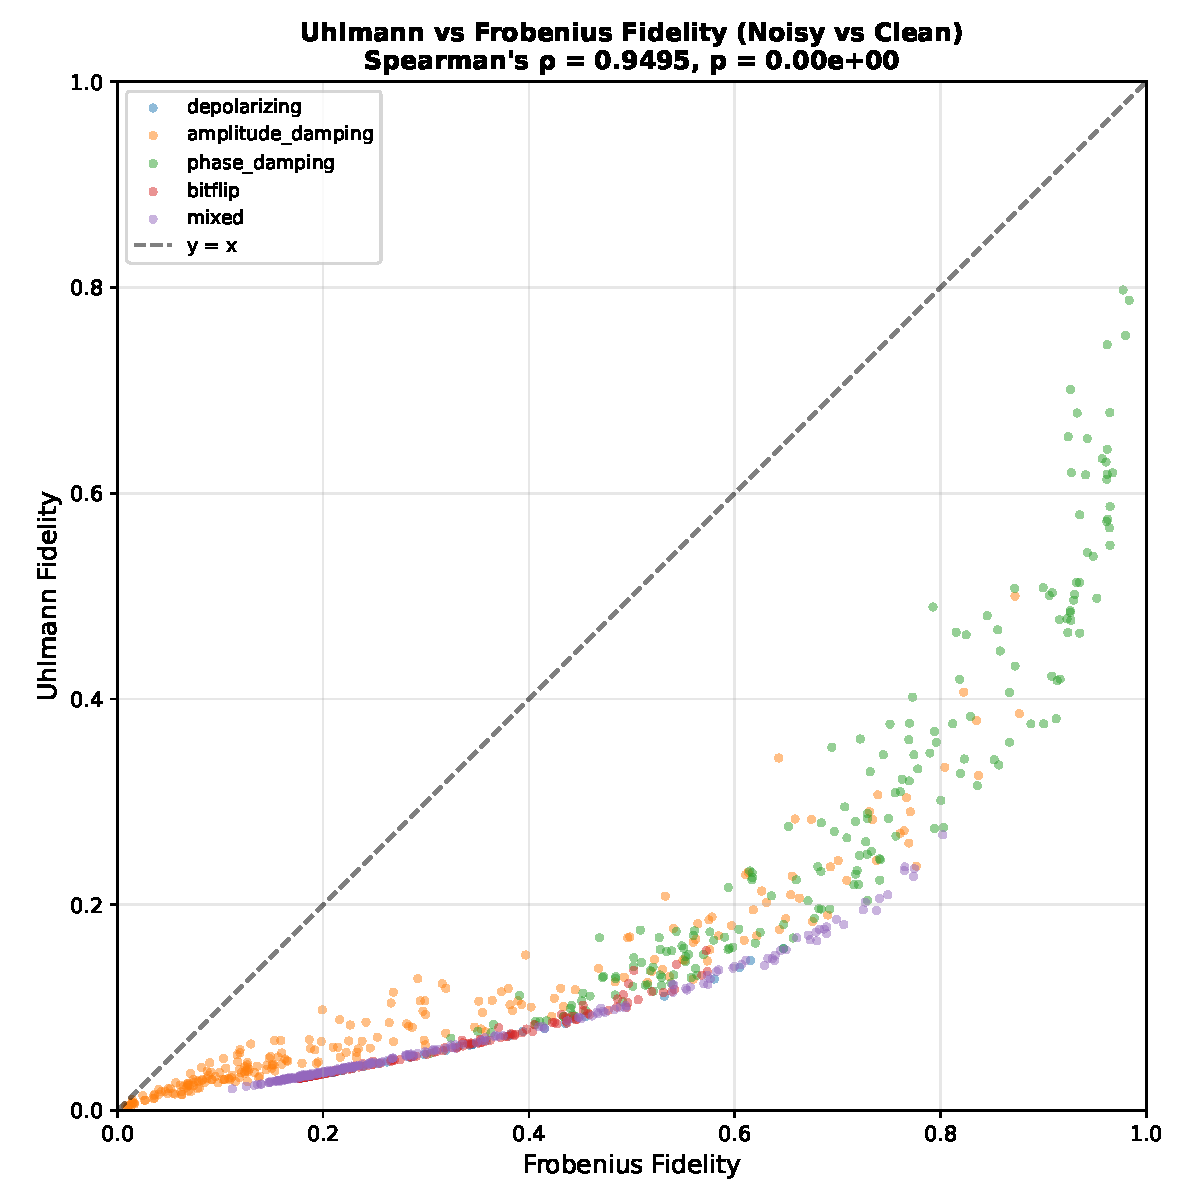
\includegraphics[width=0.8\linewidth]{./figures/uhlmann_vs_frobenius_scatter.pdf}
\caption{Relationship between normalized Frobenius similarity and Uhlmann fidelity for noisy input states.}
\label{fig:frob-uhlmann}
\end{figure}
\subsection{Normalized Frobenius Similarity Loss}
\label{sec:org9b7975d}

The reconstruction loss is a normalized Frobenius inner product measuring correlation between predicted and target density matrices:

$$
\mathcal{L}_{\text{sim}}(\hat{\rho}, \rho) = 1 - \frac{\mathrm{Re}\langle \hat{\rho}, \rho \rangle_F}{\lVert \hat{\rho} \rVert_F \cdot \lVert \rho \rVert_F}
$$

where \(\langle \hat{\rho}, \rho \rangle_F = \mathrm{Tr}(\hat{\rho}^\dagger \rho)\) is the Frobenius inner product. This formulation is analogous to cosine similarity for complex matrices: it measures alignment while normalizing for magnitude differences.

While Uhlmann fidelity is the correct operational measure of quantum state similarity, its reliance on eigendecomposition (\(O(n^3)\) for \(n \times n\) matrices) makes it substantially more expensive than the Frobenius inner product (\(O(n^2)\)). To validate Frobenius similarity as a training proxy, we computed both metrics on noisy–clean state pairs across all noise types and strengths. Although the relationship is strongly nonlinear (Figure \ref{fig:frob-uhlmann}), the two metrics exhibit a very strong monotonic association (Spearman's \(\rho = 0.95\), \(p \ll 10^{-10}\)), indicating that improvements under the Frobenius objective consistently correspond to improvements in Uhlmann fidelity. We note that the correlation appears weaker at low fidelity values where heavily corrupted states reside; however, both models successfully escape this regime during training, so the gradient signal remains informative where it matters.

\newpage
\section{Experimental Design}
\label{sec:org21760fb}
We evaluate two denoising architectures—MLP and Transformer autoencoders—with comparable parameter counts (\textasciitilde{}120k each). The architectures differ in activation functions (ReLU vs. GELU) and connectivity patterns: the MLP uses residual connections while the Transformer does not. We chose not to add residual connections to the Transformer because its encoder-decoder structure with cross-attention already preserves input information through the attention pathway, making an explicit skip connection less critical than for the MLP's severe bottleneck. Despite these differences, the similar capacity allows us to assess the relative importance of self-attention for this task. The Transformer can exploit global structure through self-attention while the MLP processes inputs as unstructured vectors with a residual bypass.

All models are trained to map noisy density matrices to their clean counterparts using unconstrained outputs with post-hoc projection to valid density matrices. Training uses the AdamW optimizer with a learning rate of 3×10⁻⁴ and light L2 regularization (weight decay 10⁻⁵). We employ early stopping with patience of 15 epochs based on validation loss, with a maximum budget of 100 epochs.

Evaluation uses Uhlmann fidelity \(F(\rho, \sigma) = (\mathrm{Tr}[\sqrt{\sqrt{\rho}\sigma\sqrt{\rho}}])^2\) between the reconstructed and target states, computed after projecting outputs to valid density matrices. Uhlmann fidelity is the standard measure of quantum state overlap, ranging from 0 (orthogonal) to 1 (identical). Computing Uhlmann fidelity requires two matrix square roots via eigendecomposition, making it expensive for training; we use Frobenius similarity as the training loss and reserve Uhlmann fidelity for evaluation.
\subsection{Hyperparameters}
\label{sec:orgcba7eb1}
\subsubsection{Shared Hyperparameters}
\label{sec:org78bf211}

\begin{center}
\begin{tabular}{ll}
Component & Value\\
\hline
Optimizer & AdamW\\
Learning rate & 3×10⁻⁴\\
Weight decay & 10⁻⁵\\
Max epochs & 100\\
Early stopping patience & 15 epochs\\
Checkpoint selection & Best validation loss\\
Dataset size & 100,000 circuits\\
Train/validation/test split & 80/10/10\\
Output constraint & Post-hoc projection\\
\end{tabular}
\end{center}
\subsubsection{Architecture-Specific Hyperparameters}
\label{sec:org6245277}

\begin{center}
\begin{tabular}{lll}
Component & MLP Autoencoder & Transformer Autoencoder\\
\hline
Input representation & Flattened 2048 (32×32×2) & 1024 element tokens (2 values each)\\
Architecture & Residual (input + correction) & Encoder-decoder\\
Hidden layers & 2048 → 28 → 28 → 2048 & —\\
Embedding dim & — & 32\\
Encoder depth & 3 linear layers & 4 layers, 4 heads\\
Decoder depth & — & 4 layers, 4 heads\\
Feed-forward dim & — & 64\\
Bottleneck & 28 dimensions & 16 dimensions (per token)\\
Batch size & 64 & 8\\
Dropout & 0.1 & 0.1\\
Activation & ReLU & GELU\\
Parameters & \textasciitilde{}117k & \textasciitilde{}119k\\
\end{tabular}
\end{center}

The MLP uses a residual architecture where the network learns corrections to the input through a 28-dimensional bottleneck, with the output layer initialized to zero so the model starts by outputting the input unchanged. The Transformer uses element-wise tokenization where each matrix element becomes a token, enabling self-attention to capture arbitrary pairwise correlations between elements—matching the non-local structure of entangled quantum states.

The smaller batch size for the Transformer accommodates the \(O(1024^2)\) attention complexity over element tokens.

We note that the two architectures differ substantially in effective latent dimensionality: the MLP compresses to 28 dimensions, while the Transformer maintains 1024 tokens with 16-dimensional per-token representations (16,384 total). This disparity is a direct consequence of architectural constraints rather than an oversight. Widening the MLP bottleneck to match the Transformer's latent capacity would increase its parameter count to over 1 million, breaking the capacity-matched comparison. Conversely, forcing the Transformer to compress through a 28-dimensional global bottleneck would defeat its core architectural advantage. The Transformer achieves higher effective dimensionality through weight-sharing: identical attention weights process all 1024 tokens, amortizing parameters across the sequence. This efficiency \emph{is} the architectural advantage we aim to study—given a fixed parameter budget, the Transformer maintains richer intermediate representations suited to the problem's non-local structure.
\subsection{Compute Resources}
\label{sec:org94a9fb9}
All experiments were conducted on a RunPod cloud instance equipped with a single NVIDIA RTX A4000 GPU (16 GB VRAM), 16 vCPUs, and 62 GB system memory. Both models fit entirely on a single GPU without gradient checkpointing or model parallelism. Training typically completed in under 100 epochs due to early stopping.
\section{Results}
\label{sec:orgf55bc70}
\subsection{Training Dynamics}
\label{sec:orgf370bd8}

\begin{figure}[htbp]
\centering
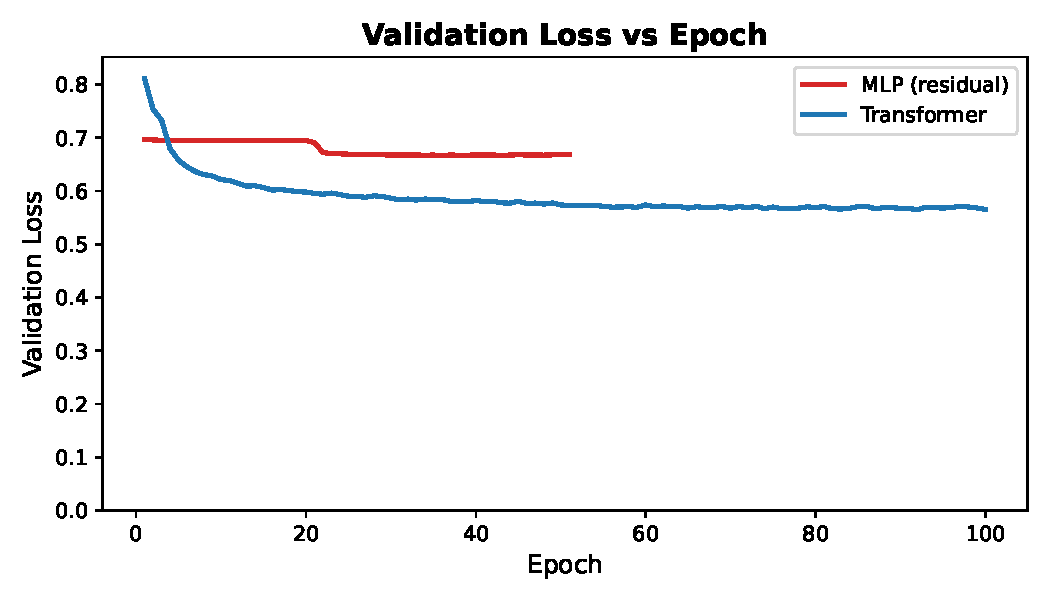
\includegraphics[width=.9\linewidth]{./figures/mlp_transformer_val_loss.pdf}
\caption{Validation loss during training. The Transformer converges rapidly to a lower loss, while the MLP plateaus at a higher value despite the residual architecture.}
\end{figure}
\subsection{Overall Performance}
\label{sec:orgf42cb5f}

Table \ref{tab:orgda8d32b} summarizes the reconstruction fidelity of both architectures compared to the baseline (noisy input without denoising).

\begin{table}[htbp]
\caption{\label{tab:orgda8d32b}Uhlmann fidelity on the held-out test set. Higher is better. Baseline represents the fidelity between noisy and clean states without any denoising.}
\centering
\begin{tabular}{lll}
Model & Uhlmann Fidelity & Improvement\\
\hline
Baseline (no denoising) & 0.12 ± 0.13 & —\\
MLP (residual) & 0.17 ± 0.17 & 1.4×\\
Transformer & 0.28 ± 0.23 & 2.3×\\
\end{tabular}
\end{table}

Both architectures improve upon the baseline, but the Transformer achieves substantially higher fidelity—1.6× better than the MLP despite having comparable parameter counts. This performance gap demonstrates that the self-attention mechanism provides a meaningful advantage for quantum state denoising, successfully exploiting the non-local correlations present in entangled states.
\subsection{Analysis}
\label{sec:org380172f}
The Transformer's advantage stems from its architectural match to the problem structure. Quantum entanglement induces correlations between arbitrary pairs of density matrix elements—precisely the kind of non-local dependency that self-attention is designed to capture. The element-wise tokenization strategy allows each matrix element to attend to every other element, enabling the model to learn which correlations are informative for denoising.

The MLP's residual architecture—learning corrections rather than full reconstruction—proves essential for feedforward denoising. Early experiments with a non-residual MLP achieved fidelity \textbf{worse} than the noisy baseline. The severe bottleneck (2048→28 dimensions) destroyed information faster than the network could learn to denoise. The residual formulation preserves input information through the skip connection, allowing the network to focus on learning corrections rather than memorizing the full state representation.

The relatively high variance in fidelity scores reflects the heterogeneity of the test set, which spans five noise types at four severity levels. Performance varies across noise conditions, with some noise types being inherently easier to correct than others.
\newpage
\subsection{Performance by Noise Type}
\label{sec:org34a2c8e}

Figure \ref{fig:noise-heatmaps} breaks down fidelity across all 20 noise conditions. Phase damping is easiest to correct—the Transformer reaches 0.71 at p=0.05, since phase damping only destroys off-diagonal coherence. Depolarizing and bit-flip noise at high levels (p=0.20) are hardest, driving states toward maximally mixed where little signal remains. The Transformer outperforms the MLP in every cell, with the largest gaps on amplitude damping and mixed noise at moderate levels.

\begin{figure}[h!]
\centering
\begin{subfigure}[b]{0.49\linewidth}
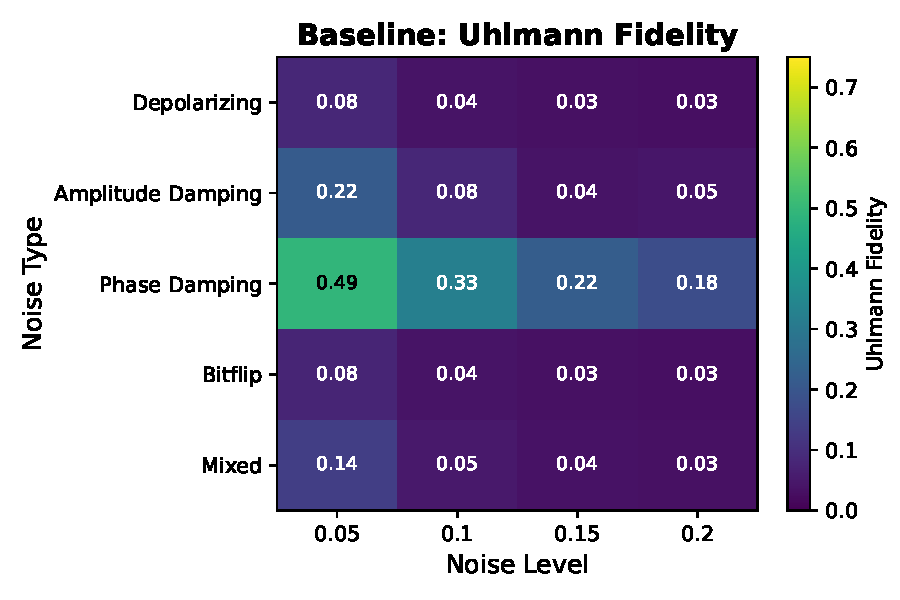
\includegraphics[width=\linewidth]{./figures/baseline_noise_cells_heatmap.pdf}
\caption{Baseline (noisy input)}
\end{subfigure}
\hfill
\begin{subfigure}[b]{0.49\linewidth}
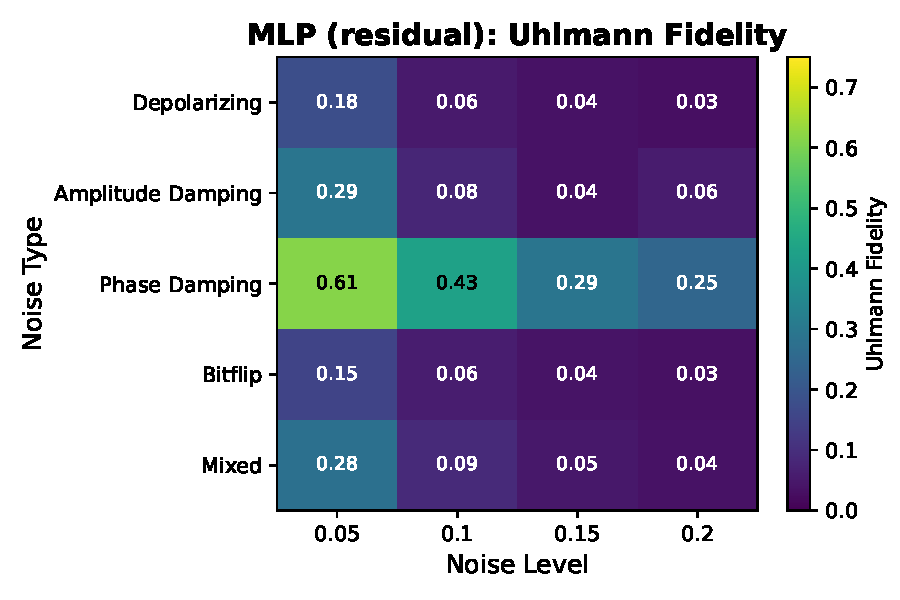
\includegraphics[width=\linewidth]{./figures/mlp_noise_cells_heatmap.pdf}
\caption{MLP (residual)}
\end{subfigure}

\vspace{0.3em}

\begin{subfigure}[b]{0.49\linewidth}
\centering
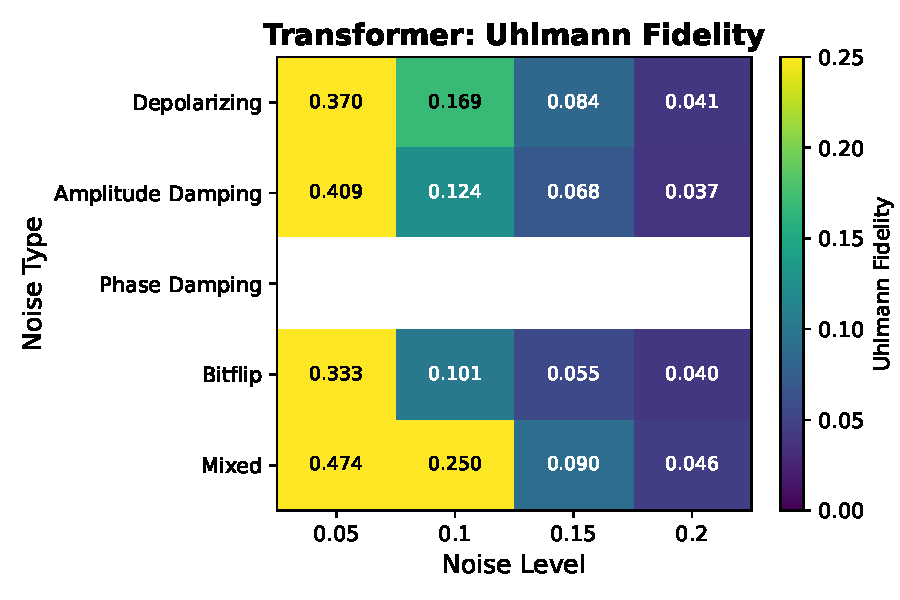
\includegraphics[width=\linewidth]{./figures/transformer_noise_cells_heatmap.pdf}
\caption{Transformer}
\end{subfigure}
\caption{Uhlmann fidelity by noise type and level. Rows: noise channels; columns: noise strength $p \in \{0.05, 0.10, 0.15, 0.20\}$.}
\label{fig:noise-heatmaps}
\end{figure}
\subsection{Attention on Entangled States}
\label{sec:org3ffa53a}

To understand \emph{why} the Transformer outperforms the MLP, we visualize what the self-attention mechanism learns. We test on a GHZ state—a standard benchmark for entanglement where all 5 qubits are correlated: measuring any one qubit instantly determines all the others. Its density matrix is nearly empty (only 4 non-zero elements out of 1024), making attention patterns easy to interpret.

Figure \ref{fig:attention} shows which tokens attend most strongly to token 0 (the \(\rho_{00,00}\) element) when processing a noisy GHZ state. Each bar represents one of the 1024 matrix elements, with height indicating attention weight.

\begin{figure}[h!]
\centering
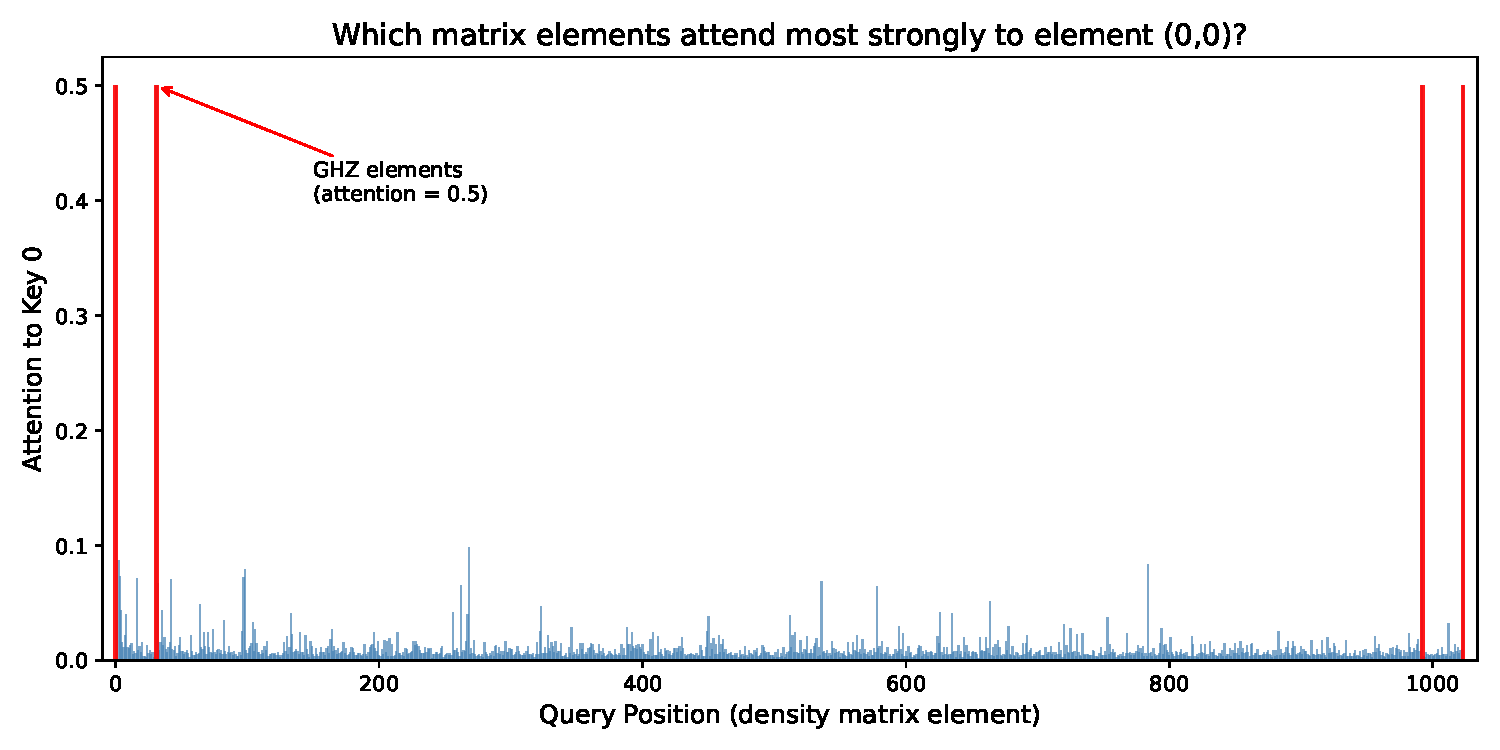
\includegraphics[width=1\linewidth]{./figures/attention_from_queries_to_key0.pdf}
\caption{Attention to token 0 (the $\rho_{00,00}$ matrix element) from all 1024 tokens. The four tall red bars at positions 0, 31, 992, and 1023 correspond exactly to the GHZ state's non-zero elements—the model learns that these specific elements should attend strongly to each other (attention weight 0.5, versus mean 0.01 for other elements).}
\label{fig:attention}
\end{figure}

The pattern is striking: the four matrix elements that are non-zero in the pure GHZ state (positions 0, 31, 992, 1023) attend to token 0 with weight 0.5—50× stronger than other elements. These correspond to the density matrix corners: \(\rho_{00,00}\), \(\rho_{00,31}\), \(\rho_{31,00}\), and \(\rho_{31,31}\). The model discovers—without explicit guidance—that these elements are correlated and should share information. This is precisely the entanglement structure: in a GHZ state, knowing one of these elements constrains the others.

\newpage
\section{Conclusion}
\label{sec:org9ba0c67}
We have demonstrated that architectural inductive bias significantly impacts neural network performance for quantum state denoising. With comparable parameter counts (\textasciitilde{}120k), the Transformer autoencoder achieves 2.3× higher Uhlmann fidelity than the noisy baseline, compared to 1.4× for the MLP—a 1.6× advantage attributable to the self-attention mechanism's ability to model correlations between arbitrary matrix elements.

Our experiments also suggest that the method of enforcing physical validity matters: unconstrained outputs with post-hoc projection to the space of valid density matrices enabled effective optimization in our setup, while hard constraints (Cholesky parameterization) led to optimization difficulties and model collapse. Whether this reflects fundamental limitations of the Cholesky approach or configuration-specific issues remains an open question.

These findings suggest that attention-based architectures may be particularly well-suited for quantum information processing tasks where non-local correlations are fundamental. The element-wise tokenization strategy—treating each density matrix element as a token—provides a natural interface between the quantum state structure and the self-attention mechanism.

The primary limitation of this work is scale: our experiments use 5-qubit systems (32×32 density matrices, 1024 tokens). The element-wise tokenization incurs \(O(n^4)\) attention complexity in qubit count (since matrix dimension scales as \(2^n\)), making naive scaling to 10+ qubits prohibitive. Future work could explore sparse attention patterns inspired by quantum locality constraints, hierarchical tokenization schemes, or hybrid architectures that maintain the benefits of self-attention while improving efficiency. Additionally, extending these methods to mixed states arising from realistic hardware noise characterization—including correlated errors and non-Markovian dynamics—could enable practical quantum error mitigation applications.
\section{References}
\label{sec:orgb67f7b4}
\noindent
Bravyi, Sergey and Cross, Andrew W. and Gambetta, Jay M. and Maslov, Dmitri and Rall, Patrick and Yoder, Theodore J. (2024). \emph{High-threshold and low-overhead fault-tolerant quantum memory}, Springer Science and Business Media LLC.

\noindent
Breuckmann, Nikolas P. and Ni, Xiaotong (2018). \emph{Scalable {Neural} {Network} {Decoders} for {Higher} {Dimensional} {Quantum} {Codes}}, Quantum.

\noindent
Bultrini, Daniel and Gordon, Max Hunter and Czarnik, Piotr and Arrasmith, Andrew and Cerezo, M. and Coles, Patrick J. and Cincio, Lukasz (2023). \emph{Unifying and benchmarking state-of-the-art quantum error mitigation techniques}, Verein zur Forderung des Open Access Publizierens in den Quantenwissenschaften.

\noindent
Cai, Zhenyu and Babbush, Ryan and Benjamin, Simon C. and Endo, Suguru and Huggins, William J. and Li, Ying and McClean, Jarrod R. and O'Brien, Thomas E. (2023). \emph{Quantum error mitigation}, American Physical Society.

\noindent
Chamberland, Christopher and Ronagh, Pooya (2018). \emph{Deep neural decoders for near term fault-tolerant experiments}, Quantum Science and Technology.

\noindent
Hanrui Wang and Pengyu Liu and Kevin Shao and Dantong Li and Jiaqi Gu and David Z. Pan and Yongshan Ding and Song Han (2023). \emph{Transformer-QEC: Quantum Error Correction Code Decoding with Transferable Transformers}.

\noindent
Karan Kendre (2025). \emph{Machine Learning for Quantum Noise Reduction}.

\noindent
Koutn\'y, Dominik and Motka, Libor and Hradil, Zden\ifmmode \check{e}\else \v{e}\fi{}k and \ifmmode \check{R}\else \v{R}\fi{}eh\'a\ifmmode \check{c}\else \v{c}\fi{}ek, Jaroslav and S\'anchez-Soto, Luis L. (2022). \emph{Neural-network quantum state tomography}, American Physical Society.

\noindent
Ma, Hailan and Qi, Bo and Petersen, Ian R and Wu, Re-Bing and Rabitz, Herschel and Dong, Daoyi (2025). \emph{Machine learning for estimation and control of quantum systems}, Oxford University Press (OUP).

\noindent
Michael A. Nielsen and Isaac L. Chuang (2010). \emph{Quantum Computation and Quantum Information: 10th Anniversary Edition}, Cambridge University Press.

\noindent
Morgillo, Angela Rosy and Mangini, Stefano and Piastra, Marco and Macchiavello, Chiara (2024). \emph{Quantum state reconstruction in a noisy environment via deep learning}, Springer Science and Business Media LLC.

\noindent
Sergey N. Filippov and Sabrina Maniscalco and Guillermo García-Pérez (2024). \emph{Scalability of quantum error mitigation techniques: from utility to advantage}.

\noindent
Volkan Erol (2025). \emph{Quantum Error Correction and Fault-Tolerant Computing: Recent Progress in Codes, Decoders, and Architectures}, Preprints.
\section{Appendix}
\label{sec:org9307681}
\subsection{Failed Experiment: Cholesky-Constrained Output Layer}
\label{sec:org702d65c}

We initially attempted to enforce physical validity of output density matrices by construction using a Cholesky decomposition output layer. The network outputs 1024 real parameters encoding a lower-triangular matrix \(L \in \mathbb{C}^{32 \times 32}\), and the density matrix is computed as \(\rho = LL^\dagger / \mathrm{Tr}(LL^\dagger)\). This guarantees Hermiticity, positive semi-definiteness, and unit trace without post-hoc projection.
\subsubsection{Architecture}
\label{sec:org061b924}

Both MLP and Transformer variants were tested:
\begin{itemize}
\item \textbf{MLP}: 2048 → 128 → 142 → 1024 with ReLU activations (\textasciitilde{}427k parameters)
\item \textbf{Transformer}: Row-based tokenization (32 rows + CLS token), 5 encoder/decoder layers, 8 heads, global projection from CLS token to 1024 Cholesky parameters (\textasciitilde{}492k parameters)
\end{itemize}
\subsubsection{Results}
\label{sec:orgcb01454}

\begin{center}
\begin{tabular}{ll}
Model & Uhlmann Fidelity\\
\hline
Baseline (noisy input) & 0.11\\
MLP Cholesky & 0.045 ± 0.018\\
Transformer Cholesky & 0.031 ± 0.003\\
\end{tabular}
\end{center}

Both Cholesky-constrained models performed \textbf{worse} than the noisy input baseline. The Transformer collapsed to outputting the maximally mixed state \(I/32\) (fidelity \(\approx 1/32 = 0.031\)), as evidenced by the near-zero standard deviation. The MLP achieved marginally higher fidelity but still degraded the input rather than denoising it.
\subsubsection{Analysis}
\label{sec:orgc8a6de4}

The Cholesky parameterization creates a highly non-convex optimization landscape. The 1024 parameters must coordinate globally to produce a valid density matrix, and small perturbations in the lower-triangular entries can cause large changes in the resulting \(\rho = LL^\dagger\). This appears to make gradient-based optimization difficult, with models converging to trivial solutions (maximally mixed state) rather than learning meaningful denoising.

We abandoned this approach in favor of unconstrained outputs with post-hoc projection to the space of valid density matrices.
\end{document}
